%%%%%%%%%%%%%%%%%%%%%%%%%%%%%%%%%%%%%%%%%%%%%%%%%%%%%%%%%%%%%%%%%%%%%%%%%%%%%%%%%%%%
% Document data
%%%%%%%%%%%%%%%%%%%%%%%%%%%%%%%%%%%%%%%%%%%%%%%%%%%%%%%%%%%%%%%%%%%%%%%%%%%%%%%%%%%%
\documentclass[12pt]{article}
%%%%%%%%%%%%%%%%%%%%%%%%%%%%%%%%%%%%%%%%%%%%%%%%%%%%%%%%%%%%%%%%%%%%%%%%%%%%%%%%%%%%




%%%%%%%%%%%%%%%%%%%%%%%%%%%%%%%%%%%%%%%%%%%%%%%%%%%%%%%%%%%%%%%%%%%%%%%%%%%%%%%%%%%%
% Packages
%%%%%%%%%%%%%%%%%%%%%%%%%%%%%%%%%%%%%%%%%%%%%%%%%%%%%%%%%%%%%%%%%%%%%%%%%%%%%%%%%%%%
\usepackage{color, soul, xcolor} % Colored text and highlighting, respectively
\usepackage{tikz-cd} % For commutative diagrams
\usepackage{mathtools}
\usepackage{answers}
\usepackage{setspace}
\usepackage{graphicx}
\usepackage{enumerate}
\usepackage{multicol}
\usepackage{mathrsfs}
\usepackage[margin=1in]{geometry} 
\usepackage{amsmath,amsthm,amssymb}
\usepackage{marvosym,wasysym} %fucking smileys
%%%%%%%%%%%%%%%%%%%%%%%%%%%%%%%%%%%%%%%%%%%%%%%%%%%%%%%%%%%%%%%%%%%%%%%%%%%%%%%%%%%%




%%%%%%%%%%%%%%%%%%%%%%%%%%%%%%%%%%%%%%%%%%%%%%%%%%%%%%%%%%%%%%%%%%%%%%%%%%%%%%%%%%%%
% Shortcuts
%%%%%%%%%%%%%%%%%%%%%%%%%%%%%%%%%%%%%%%%%%%%%%%%%%%%%%%%%%%%%%%%%%%%%%%%%%%%%%%%%%%%
% Number systems
\newcommand{\N}{\mathbb{N}}
\newcommand{\Z}{\mathbb{Z}}
\newcommand{\C}{\mathbb{C}}
\newcommand{\R}{\mathbb{R}}
\newcommand{\Q}{\mathbb{Q}}

% Operators/functions
\newcommand{\id}{\mathrm{Id}}
\DeclareMathOperator{\sech}{sech}
\DeclareMathOperator{\csch}{csch}
%%%%%%%%%%%%%%%%%%%%%%%%%%%%%%%%%%%%%%%%%%%%%%%%%%%%%%%%%%%%%%%%%%%%%%%%%%%%%%%%%%%%




%%%%%%%%%%%%%%%%%%%%%%%%%%%%%%%%%%%%%%%%%%%%%%%%%%%%%%%%%%%%%%%%%%%%%%%%%%%%%%%%%%%%
% Environments
%%%%%%%%%%%%%%%%%%%%%%%%%%%%%%%%%%%%%%%%%%%%%%%%%%%%%%%%%%%%%%%%%%%%%%%%%%%%%%%%%%%%
% Italic font
\newtheorem{theorem}{Theorem}[section]
\newtheorem{lemma}{Lemma}[section]
\newtheorem{corollary}{Corollary}[section]

% Plain font
\theoremstyle{definition}
\newtheorem{definition}{Definition}[section]
\newtheorem{example}{Example}[section]
\newtheorem{remark}{Remark}[section]
\newtheorem{solution}{Solution}[section]
\newtheorem{problem}{Problem}[section]
\newtheorem{question}{Question}[section]
\newtheorem{answer}{Answer}[section]
%%%%%%%%%%%%%%%%%%%%%%%%%%%%%%%%%%%%%%%%%%%%%%%%%%%%%%%%%%%%%%%%%%%%%%%%%%%%%%%%%%%%
 
 
 
%%%%%%%%%%%%%%%%%%%%%%%%%%%%%%%%%%%%%%%%%%%%%%%%%%%%%%%%%%%%%%%%%%%%%%%%%%%%%%%%%%%%
% Beginning of document
%%%%%%%%%%%%%%%%%%%%%%%%%%%%%%%%%%%%%%%%%%%%%%%%%%%%%%%%%%%%%%%%%%%%%%%%%%%%%%%%%%%%
\begin{document}
 
\title{Just In Time Session}
\maketitle
%%%%%%%%%%%%%%%%%%%%%%%%%%%%%%%%%%%%%%%%%%%%%%%%%%%%%%%%%%%%%%%%%%%%%%%%%%%%%%%%%%%%


\section{Pre-Calculus}

This section should largely be a review.  Make sure these topics are all very comfortable for you.

\subsection{Trigonometric Functions}

For each function, we will use the following figure:
\begin{figure}[h]
    \centering
    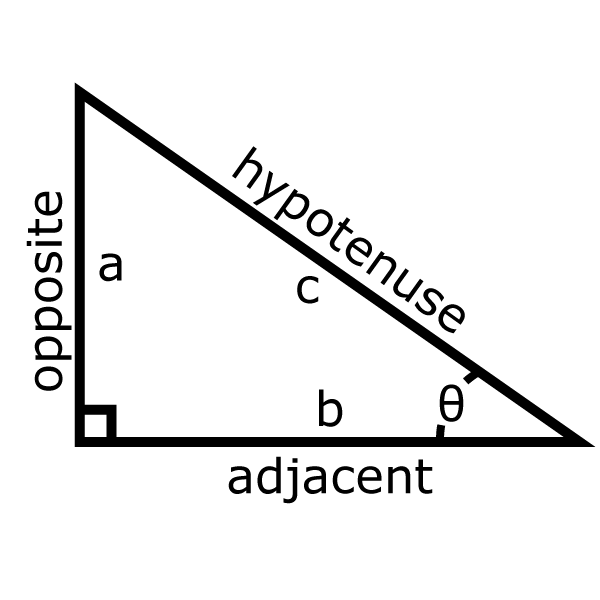
\includegraphics[scale=0.2]{right_triangle.png}
    \caption{A right triangle with angle $\theta$.}
    \label{fig:right_triangle}
\end{figure}

We define
\begin{itemize}
    \item $\sin \theta = \frac{a}{c},$
    \item $\cos \theta = \frac{b}{c},$
    \item $\tan \theta = \frac{a}{b}$.
\end{itemize}

\begin{problem}
Plot each of these as a function of $\theta$.  Notice where any discontinuities happen.  Where are they?
\end{problem}

\subsection{Exponentials and Logarithms}

An \textbf{exponential function with base $a$} is given by
\[
f(x)=a^x.
\]

Recall the following:

\begin{center}
\begin{tabular}{cc}
    Law 1: & $a^x\cdot a^y = a^{x+y}$\\
    Law 2: & $(a^x)^y=a^{xy}$\\
    Law 3: & $a^{-x}=\frac{1}{a^x}$\\
    Law 4: & $\frac{a^y}{a^x}=a^{y-x}$\\
    Law 5: & $a^1=a$\\
    Law 6: & $a^0=1$.
\end{tabular}
\end{center}

\begin{problem}
Verify each one of these rules using the fact that we have
\[
a^x = \underbrace{a\cdot a \cdots a}_{\textrm{$x$ times}}. 
\]
If you go in order from 1-6, this should be doable.
\end{problem}

An important number to know is Euler's number
\[
e\approx 2.7183.
\]
If you're wondering where the exact number comes from, check Wikipedia. Of course, $e^x$ follows all the usual laws for exponential functions.

\begin{definition}
The inverse function to the exponential function $e^x$ is $\ln x$.  In other words, we have
\begin{align*}
    \ln(e^x)&=x\\
    e^{\ln x}&=x.
\end{align*}
\end{definition}

Recall the following:

\begin{center}
\begin{tabular}{cc}
    Law 1: & $\ln (xy) = \ln x + \ln y$\\
    Law 2: & $\ln(x^y)=y\ln x$\\
    Law 3: & $\ln(1/x)=-\ln x$\\
    Law 4: & $\ln(x/y)=\ln x - \ln y$\\
    Law 5: & $\ln e =1$\\
    Law 6: & $\ln 1 = 0$.\\
    Law 7: & $\log_a (x) = \frac{\ln x}{\ln a}.$
\end{tabular}
\end{center}

\begin{problem}
Verify these rules by using the fact that the natural log is the inverse to the exponential function. Take the time to understand why these really must be true.
\end{problem}

\begin{example}[Semilog Plots]
Say we have the functions
\begin{align*}
    S(t)&=150e^{1.2t}\\
    M(t)&=13.2e^{2t}.
\end{align*}
Plotting both of these in their respective planes ($S$ vs. $t$ and $M$ vs. $t$) then we get an exponential function curve.  However, these can be a bit harder to interpret certain values, like where the curves intersect.

Instead, we can plot these in a \textbf{semilog} graph.  Meaning we plot $\ln S$ vs $t$ and $\ln M$ vs $t$. So, in this case
\begin{align*}
    \ln S(t)&=\ln(150e^{1.2t})\\
    &= \ln 150 + 1.2t
\end{align*}
and
\begin{align*}
    \ln M(t)&=\ln 13.2 + 2t.
\end{align*}
Now these are both linear equations which are much easier to handle.
\end{example}

\begin{example}[Double Log Plots]
Consider the function
\[
y=cx^p.
\]
Then, taking log of both sides yields
\[
\ln y = \ln c + p \ln x,
\]
and we can plot this as a line with slope $p$ and intercept $c$.  
\end{example}

\section{Derivatives}

\subsection{Definition and Intuition}

\begin{question}
What was Newton's motivation for the derivative? What do we mean by derivative? Where does it show up in physics? 
\end{question}

\begin{answer}~
\begin{itemize}
    \item When studying the physical world, knowing how a system changes is of vital importance for understanding kinematics, mechanics, and dynamics.  Hence, Newton needed to have a rigorous notion of change. Specifically, how some quantity would change at a single point in time as opposed to over an interval in time.
    \item The word ``derivative" should make you think ``instantaneous rate of change."  If we look at some function $f$, we can zoom in on a single point $x_0$ in doing this we find that every (sufficiently nice) function looks linear.  It is the slope of this linear approximation that tells us the instantaneous rate of change of $f$ at the point $x_0$. We denote this $f'(x_0)=\left. \frac{d}{dx}f(x) \right|_x=x_0$.  Other notations may show up.
    \item It would likely be easier to list the places in physics where derivatives \emph{don't} show up.  Any system that changes over time will have the time derivative show up. Even static systems can be understood by setting derivatives equal to zero.
    
    A few explicit examples: Kinematic equations, mechanics, electrodynamics, waves, and quantum mechanics.
\end{itemize}
\end{answer}

\begin{example}[Secant Line]
Any function $f$ defined on an open interval admits a \textbf{secant line approximation}.  Take the following function defined on all of $\R$:
\[
f(x)=x^3.
\]
Take the points $x_1=-1$ and $x_2=0$. Then the secant line between these points is
\begin{align*}
y&=\frac{f(x_2)-f(x_1)}{x_2-x_1}(x-x_1)+f(x_1)\\
&=x.
\end{align*}
Be sure you can verify this for yourself.
\end{example}

\begin{problem}
Find the secant line of $f(x)=x^3$ with the points $x_1=-1/2$ and $x_2=1/2$.
\end{problem}


Take a look at the graph from the above example
\begin{figure}[h]
    \centering
    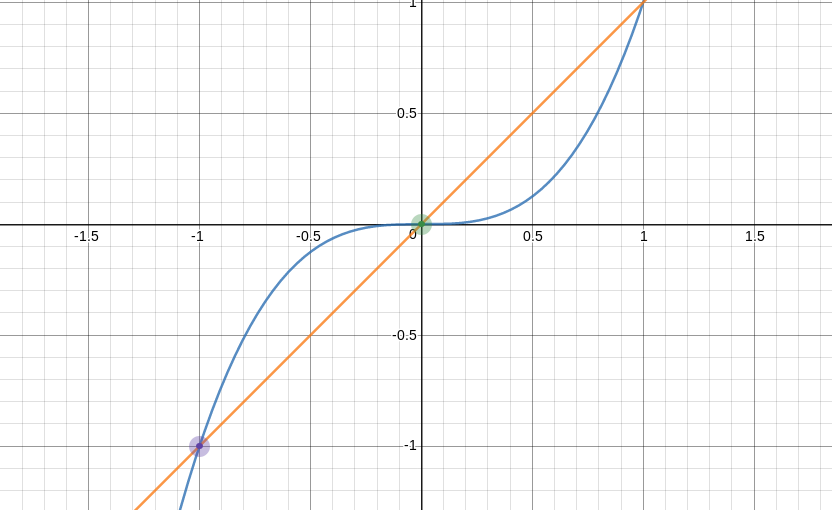
\includegraphics[scale=.3]{secant_line_1.png}
    \caption{Graph of $f(x)=x^3$ and a secant line approximation with points $x_1=-1$ and $x_2=0$.}
    \label{fig:secant_line_1}
\end{figure}

\begin{question}
As we move $x_2$ closer to $x_1$, what can we say about the secant line through these points for the function $f$?
\end{question}

\begin{answer}
The secant line will approach the tangent line to the function $f$ at the point $x_1$.
\end{answer}

It's worth seeing this graphically. Instead of $x_1=-1$ and $x_2=0$, we move $x_2$ much closer. So we let $x_1=-1$ and $x_2 = -0.9$.
\begin{figure}[h]
    \centering
    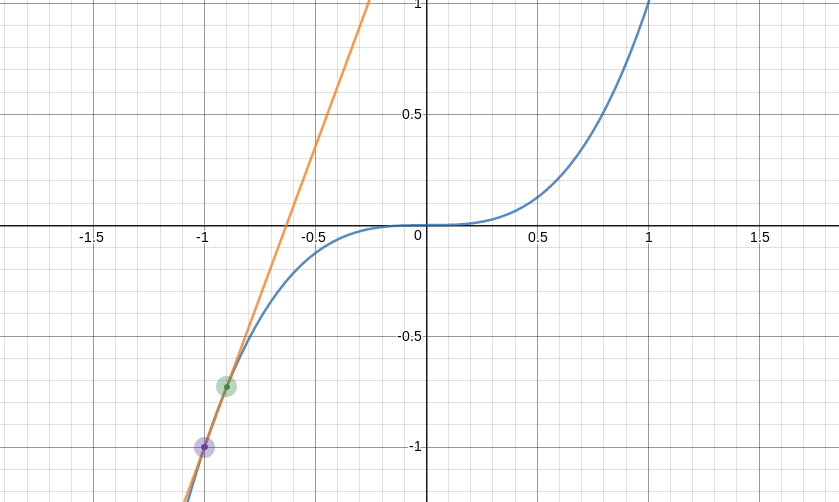
\includegraphics[scale=.3]{secant_line_2.png}
    \caption{Graph of $f(x)=x^3$ and a secant line approximation with points $x_1=-1$ and $x_2=-0.9$.}
    \label{fig:secant_line_2}
\end{figure}

Let us pause for a second in order to think about what we're doing.  We've defined a secant line approximation to a function, but why?
\begin{question}
What is the physical interpretation for a secant line approximation, say, of a function $f$ with the points $x_1$ and $x_2$?
\end{question}

\begin{answer}
It is the average rate of change of $f$ on the interval $[x_1,x_2]$. 
\end{answer}

\begin{question}
Seeing that the secant line gives us an \emph{average rate of change of $f$} over an interval, what if we let the size of this interval we average over shrink to a single point?
\end{question}

\begin{answer}
We will find a tangent line at the single point which corresponds to an average rate of change at a single point which we interpret as an \emph{instantaneous rate of change of $f$} at that point.
\end{answer}

Recall that we found the slope of a secant line of $f$ with points $x_1$ and $x_2$ by
\[
\frac{f(x_2)-f(x_1)}{x_2-x_1}.
\]
We wish to let $x_2$ approach $x_1$ and get as close as possible, which motivates the following definition.

\begin{definition}[Slope of Tangent Line]
Let $f$ be defined on an interval $(a,b)$ that contains the point $x_0$. Then the \textbf{slope of the tangent line to $f$ at the point $x_0$} (denoted $f'(x_0)$) is given by
\[
f'(x_0)\coloneqq\lim_{x\to x_0} \frac{f(x)-f(x_0)}{x-x_0},
\]
when the limit exists. When the limit exists, we say that $f$ is \textbf{differentiable}.
\end{definition}

\begin{remark}
In physics, $f$ will almost always be differentiable.  We tend to take this for granted.
\end{remark}

\begin{problem}
Verify that the definition
\[
f'(x_0)=\lim_{h\to 0} \frac{f(x_0+h)-f(x_0)}{h},
\]
is equivalent to the given definition.
\end{problem}

\begin{example}
Consider the function $f(x)=x^2.$  Let us find the slope of the tangent line to $f$ at the point $x_0$. We have
\begin{align*}
    f'(x_0)&=\lim_{x\to x_0} \frac{f(x)-f(x_0)}{x-x_0}\\
    &= \lim_{x\to x_0} \frac{x^2-x_0^2}{x-x_0}\\
    &= \lim_{x\to x_0} \frac{(x-x_0)(x+x_0)}{x-x_0}\\
    &= \lim_{x\to x_0} x+x_0\\
    &= 2x_0.
\end{align*}
\end{example}

\begin{remark}
It's worth noting that $x_0$ was arbitrary.  This should make you realize that we now have this new function $f'$ that tells us the slope of the tangent line to $f$ at a point $x_0$.
\end{remark}

\begin{definition}[Derivative]
If $f$ is differentiable on $(a,b)$, then $f'(x)$ exists on $(a,b)$ as well.  We call $f'(x)$ the \textbf{derivative} of $f$.
\end{definition}

\begin{remark}
We often write the following:
\[
f'(x)=\frac{d}{dx} f(x),
\]
where we think of $\frac{d}{dx}$ as \emph{operating} on the function $f$ and returning the function $f'$. The notation is more or less interchangeable and you will also see $f'(x)=\frac{df}{dx}.$
\end{remark}

\subsection{Derivative Rules}

\subsubsection{Rules for Functions in General}

We have four main results for the derivative of functions.  From here on out, we assume that all functions mentioned are differentiable everywhere needed. Extra requirements will be stated. Proofs for these statements are not given here, but are readily available online if you desire. Or you can prove each statement yourself!

\begin{theorem}[Linearity of the Derivative Operation]
The derivative operation $\frac{d}{dx}$ (or $'$) is \textbf{linear}. That is to say, for $f,g$ functions and $a,b$ real (even complex) numbers, we have
\[
(af+bg)'(x)=\frac{d}{dx}(af+bg)(x)=a\frac{df}{dx}(x)+b\frac{dg}{dx}(x)=af'(x)+bg'(x).
\]
\end{theorem}

\begin{remark}
This is often broken into the \emph{constant multiple rule}: 
\[
\frac{d}{dx}(af)(x)=a\frac{df}{dx}(x),
\]
and the \emph{sum} rule:
\[
\frac{d}{dx}(f+g)(x)=\frac{df}{dx}(x)+\frac{dg}{dx}(x).
\]
Saying that $\frac{d}{dx}$ is \emph{linear} takes care of both of these.
\end{remark}

\begin{theorem}[Product Rule for the Derivative Operation]
The derivative of a product of functions $(fg)(x)=f(x)g(x)$ follows the \textbf{product (or Leibiniz) rule}:
\[
(fg)'(x)=\frac{d}{dx}(fg)(x)=\frac{df}{dx}(x)g(x)+f(x)\frac{dg}{dx}(x)=f'(x)g(x)+f(x)g'(x).
\]
\end{theorem}

\begin{theorem}[Quotient Rule for the Derivative Operation]
The derivative of the quotient of two functions $(f/g)(x)=f(x)/g(x)$ (where, of course, $g(x)\neq 0$) follows the \textbf{quotient rule}:
\[
(f/g)'(x)=\frac{d}{dx}(f/g)(x)=\frac{\frac{df}{dx}(x)g(x)-f(x)\frac{dg}{dx}(x)}{g(x)^2}=\frac{f'(x)g(x)-f(x)g'(x)}{g(x)^2}.
\]
\end{theorem}

\begin{theorem}[Chain Rule for the Derivation Operation]
The derivative of the composition of two functions $(g\circ f)(x)=g(f(x))$ follows the \textbf{chain rule}:
\[
(g\circ f)'(x)=\frac{d}{dx}(g\circ f)(x)=\frac{dg}{dx}(f(x))\cdot\frac{df}{dx}(x)=g'(f(x))\cdot f'(x).
\]
\end{theorem}

\begin{problem}
Write the chain rule for the composition of three functions $(h\circ g \circ f)(x)$.
\end{problem}

\begin{theorem}[Power Rule for the Derivative Operation]
Let $f(x)=x^r$ where $r$ is any real number.  Then the \textbf{power rule} says that
\[
f'(x)=\frac{d}{dx}f(x)=rx^{r-1}.
\]
\end{theorem}

\begin{problem}
Derive the quotient rule from the product and power rules.
\end{problem}


\subsubsection{Common Derivatives}

\begin{itemize}
    \item $f(x)=\sin x$, then $f'(x)=\cos x.$
    \item $f(x)=\cos x$, then $f'(x)=-\sin x$. The relationship between $\sin$ and $\cos$ is important.
    \item $f(x)=\tan x$, then $f'(x)=\sec^2 x$.
    \item $f(x)=e^x$, then $f'(x)=e^x$. This is very special.
    \item $f(x)=a^x$, then $f'(x)=a^x \ln(a)$. (See problem below.)
    \item $f(x)=\ln x$, then $f'(x)=\frac{1}{x}$. 
    \item $f(x)=\log_a(x)$, then $f'(x)=\frac{1}{x\ln a}.$ (See problem below.)
\end{itemize}

\begin{problem}~
\begin{itemize}
    \item Verify that $\frac{d}{dx}(a^x)=a^x \ln(a)$ by using log rules.  (Hint: note that $e^{\ln(a^x)}=a^x$.)
    \item Verify that $\frac{d}{dx}(\log_a(x)=\frac{1}{x\ln a}$ by using log rules. (Hint: $\log_a(x)=\frac{\ln x}{\ln a}$.)
\end{itemize}
\end{problem}

\begin{problem}
Find the derivatives for $\sec$, $\csc$, and $\cot$ using the derivative rules and common derivatives.
\end{problem}

\section{Integration}

\begin{question}
What is the physical motivation for an integral? What do we mean by evaluating an integral? Where does it show up in physics?
\end{question}

\begin{itemize}
    \item The motivating idea behind the integral is that we can add up infinitesimal changes to a system. By doing this, we can better understand systems that are changing continuously in time. Take for example, wind blowing a leaf over some time.  The speed of the leaf could be found by integrating the force from the air over time.
    \item By evaluating an integral, we mean that we have found the signed area under a curve.  This area under a curve can have many different physical implications.
    \item Again, it would be easier to list the places where you don't find integrals.  Take the following examples: Work, impulse, flux, moments of inertia, actions, and probability.
\end{itemize}

\begin{definition}[Riemann Sum]
Any function defined on an closed interval admits a \textbf{(left, right, or midpoint) Riemann sum}. Take the function $f(x)$ defined on $[a,b]$. We break (\emph{partition}) $[a,b]$ into $n$ equal segments. So we let $a=x_0$, $b=x_n$, so we have the following segments $[x_0,x_1],\dots,[x_{n-1},x_n]$ so that $[a,b]=[x_0,x_1]\cup \cdots \cup [x_{n-1},x_n]$. Then we define the following:
\begin{itemize}
    \item The \textbf{left Riemann sum over the partition} is
    \[
    S_{left}=\sum_{i=0}^{n-1}f(x_i) \frac{b-a}{n}.
    \]
    \item The \textbf{right Riemann sum over the partition} is
    \[
    S_{right}=\sum_{i=1}^n f(x_i) \frac{b-a}{n}.
    \]
\end{itemize}
\end{definition}

\begin{remark}
It is very helpful to note that the quantity $\frac{b-a}{n}$ can be regarded as the width of each subinterval when they're constant.  In that case, we can denote $\Delta x \coloneqq \frac{b-a}{n}$.
\end{remark}

\begin{problem}
Define the midpoint Riemann sum in an analogous way.
\end{problem}

Seeing what this looks like is arguably far more appealing than the definition above.  So, lets see this. 

\begin{example}[Visual of Left and Right Riemann Sums]
Take $f(x)=x+1$ defined on the interval $[0,1]$.  We partition $[0,1]$ into 10 evenly sized intervals $[0,0.1],[0.1,0.2],\dots,[0.9,1]$.  The left Riemann sum over this partition adds the area of the rectangles in the following figure
\begin{figure}[h]
    \centering
    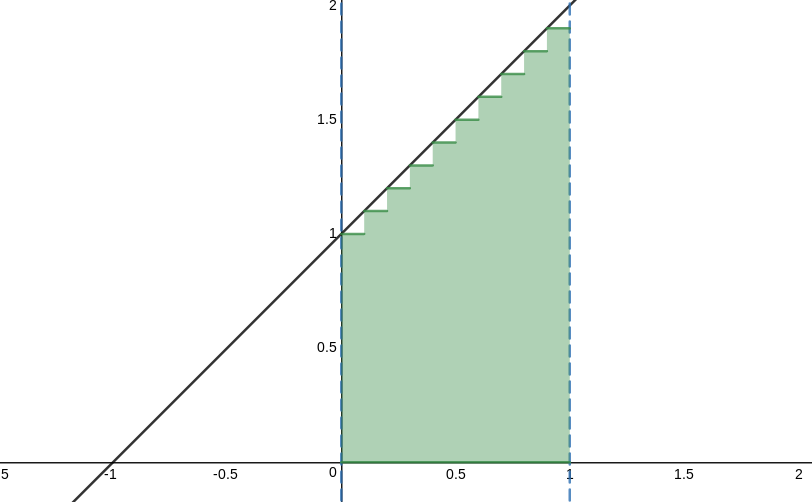
\includegraphics[scale=.3]{left_riemann.png}
    \caption{An illustration of the left Riemann sum.}
    \label{fig:left_riemann}
\end{figure}
Similarly, the right Riemann sum over this partition adds the area of the rectangles in the following figure
\begin{figure}[h]
    \centering
    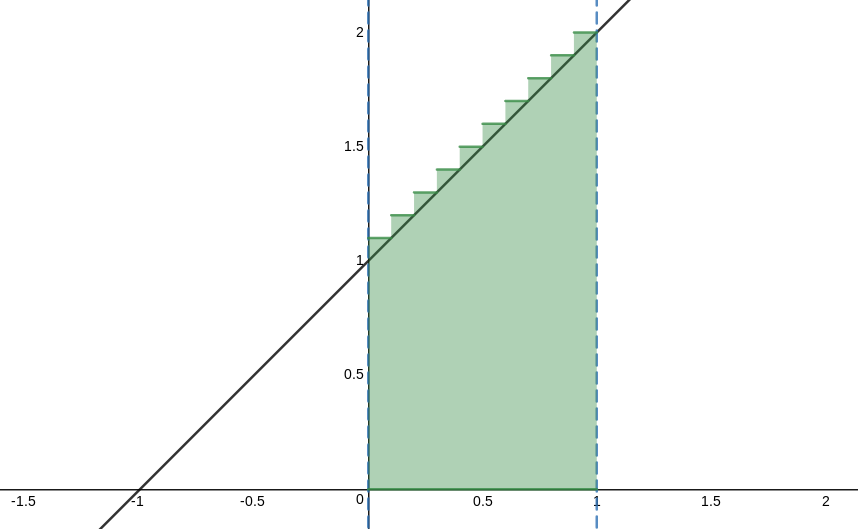
\includegraphics[scale=.3]{right_riemann.png}
    \caption{An illustration of the right Riemann sum.}
    \label{fig:right_riemann}
\end{figure}
\end{example}

\begin{problem}
Calculate the left and right Riemann sums in the previous example. Compare their values.  Which is larger and why?
\end{problem}

In a manner that is analogous to moving from a secant line to a tangent line, we can take Riemann sums to integrals. 

\begin{definition}[Integral]
Let $f$ be a function defined on the interval $[a,b]$. Partition $[a,b]$ into $n$ equally sized (of width $\Delta x = \frac{b-a}{n}$) subintervals as before.  Then we define the \textbf{integral of $f$ from $a$ to $b$} by
\[
\int_a^b f(x) dx \coloneqq \lim_{n\to \infty} \sum_{i=0}^n f(x_i) \Delta x.
\]
This is to say that we want to find the limit as the size of each subinterval goes to zero for (any) Riemann sum. When this limit is defined, we say that $f$ is \textbf{integrable on $[a,b]$}. 
\end{definition}

\begin{remark}
It does not matter which type (left, right, midpoint, or other) Riemann sum you use since the size of each subinterval will ultimately be a single point. Intuitively, we let $\Delta x \to dx$, where $dx$ can be thought of as an \emph{infinitesimal} (i.e., the smallest possible distance between real numbers).
\end{remark}

What comes next is a brief digression on notation.  The next few pieces of information are not critical, but are supplemental in understanding calculus further.

\begin{question}
What is $dx$? 
\end{question}

\begin{answer}
This is a commonly recurring question that can take you down a rabbit hole of pure mathematics. The honest answer: $dx$ is a \emph{differential 1-form}.  

However, the way you should think about $dx$ is two fold.
\begin{itemize}
    \item $dx$ is an infinitesimal quantity.  In some sense, $x+dx$ would give you the ``next" real number after $x$.  On an intuitive level, this is totally okay to think.  Just be weary of the fact that there is not really a ``next" real number (hence the quotes).
    \item $dx$ is a function. This is to say that $dx(x_0)$ has some value.  The value that it outputs is not really important to us since, for all of our cases, it will be constant. 
\end{itemize}
\end{answer}

\begin{question}
What is $df$?
\end{question}

\begin{answer}~
\begin{itemize}
    \item First and foremost, it is a way of representing an infinitesimal change in a function $f$. In 1-dimension, at every point $x$
    \[
    df(x)\propto dx(x),
    \]
    where the constant of proportionality we write down is usually denoted $f'(x)$. This proportion is \emph{exactly} the slope of the tangent line to $f$.
    
    \item In higher dimensions, say two, we instead have
    \[
    df(\vec{x}) = \frac{\partial f}{\partial x}dx(\vec{x})+\frac{\partial f}{\partial y}dy(\vec{x}).
    \]
    Right now, this is not essential in any way.  This is just to de-mystify the symbols being used. (Note that $\frac{\partial f}{\partial x}$ are partial derivatives of a function $f(x,y)$.)
\end{itemize}
\end{answer}

\begin{problem}
Pick an $f$. At some point $x$ and a nearby point find $\Delta x$ and $\Delta f$ for a secant line. Let $\Delta x \to 0$. (Consider trying this with Desmos. They have a secant line demo.) We don't get lucky with the proportionality in higher dimensions, and calculus changes a bit.
\end{problem}

\begin{remark}
The notation $\frac{df}{dx}$ is really a ratio of two functions (by the above answer).  What is it saying?  Well, it is saying, ``how much does our output $f$ change with respect to an input $x$?" This is \underline{exactly} the definition of the derivative we know.  It's worth noting, but not dwelling on, the fact that we should say
\begin{align*}
    df&=f'dx,
\end{align*}
where $f'$ is the ratio of the change of the output with respect to the change in input.  If we divide by the function $dx$, we see
\[
\frac{df}{dx}=f'.
\]
This may be very foreign.  That's fine if it is the case. But this is where the notation comes from, and it's worth seeing at least once in your life.  

We call $df$ the \emph{differential of $f$}, and it is a quantity that shows up in MATH 261 when you have to do a bit more work to define the derivative (Jacobian, or differential).
\end{remark}

\subsection{Antiderivatives and the Fundamental Theorem of Calculus (Stokes' Theorem)}

There are a few things to be said about evaluating integrals.
\begin{itemize}
    \item Integrable functions can be very badly behaved.  They need not be continuous, let alone differentiable.
    \item When integrating differentiable functions, we have nicer analytical results.
\end{itemize}

\begin{problem}
Find a discontinuous function and an interval where you can evaluate the integral of the function you chose.
\end{problem}

\begin{theorem}[Fundamental Theorem of Calculus]
If $f$ is a differentiable function on $[a,b]$ with derivative $f'$, then we have
\[
\int_a^b f'(x)dx = f(b)-f(a).
\]
\end{theorem}

\begin{remark}
In MATH 261, you will talk about Stokes' theorem and Gauss's theorem.  These are higher dimensional analogs to the Fundamental Theorem of Calculus.  In fact, there is one for each dimension $n$.  In general, we refer to these all as Stokes' theorem and the $1$-dimensional case is the Fundamental Theorem of Calculus.
\end{remark}

\begin{problem}
Define
\[
F(x)=\int_a^x f(\tilde{x})d\tilde{x}.
\]
Describe what $F(x)$ is.  What is $F'(x)$?
\end{problem}

\begin{definition}[Antiderivative]
If $f$ is differentiable on the real numbers $\R$, then we define the \textbf{antiderivative of $f$} as
\[
F(x)=\int f(x)dx.
\]
Then, by the Fundamental Theorem of Calculus, we have
\[
F'(x)=f(x).
\]
\end{definition}

\begin{remark}
$F(x)$ is determined only up to a constant real number $C$ since
\[
\frac{d}{dx}(F(x)+C)=\frac{dF}{dx}(x)+\frac{dC}{dx}=\frac{dF}{dx}(x)=f(x).
\]
In other words, $F(x)$ is an infinite family of functions.
\end{remark}

\begin{problem}
Using the derivative rules and the Fundamental Theorem of Calculus, evaluate
\[
\int_1^5 3x^2+e^x dx.
\]
\end{problem}

\begin{remark}
More or less, we can say that
\begin{align*}
    \frac{d}{dx} \int f(x) dx &= f(x)
\end{align*}
and
\[
\int \frac{d}{dx}f(x)dx=f(x).
\]
This shows that the derivative and antiderivative are inverse operations.
\end{remark}

\subsection{Integration Techniques}

Above all else, the fundamental theorem of calculus is the most useful integral technique. You will find that many times you can find an antiderivative of a function and evaluate this at the endpoints of the interval to find the value of the integral.  

\subsubsection{Change of Variables or the $u$-Substitution}

Often times we run into an integral where we can't immediately find an antiderivative.  However, we can still have some hope of slightly modifying the integral in order to work it out analytically.

\begin{theorem}[Change of Variables]
Let $f(x)$ be defined on $[a,b]$.  Then for a differentiable function $\varphi(x)$ defined on $[c,d]$ with $\varphi(c)=a$ and $\varphi(d)=b$, we have
\begin{align*}
    \int_a^b f(u)du &= \int_c^d f(\varphi(x))\frac{d\varphi}{dx}dx.
\end{align*}
\end{theorem}

This way of writing the theorem down is often slightly confusing.  Let's instead concentrate on an example:

\begin{example}[Change of Variables with a $u$-Substitution]
We want to evaluate:
\[
\int_0^{\pi/2} \sin x \cos x dx.
\]
Here we let $u=\sin x$ so that $du=\cos x dx$.  Now $\sin 0=0$ and $\sin (\pi/2) = 1$.  We then have
\begin{align*}
    \int_0^1 udu &= \left. \frac{1}{2}u^2 \right|_0^1\\
    &= \frac{1}{2}.
\end{align*}
\end{example}

\begin{remark}
In the example, we started with an integral in the form:
\[
\int_a^b f(\varphi(x))\varphi'(x)dx.
\]
We let $f(x)=x$, and $\varphi(x)=\sin x$ so that $\varphi'(x)=\cos x$.  
\end{remark}

\begin{problem}
Verify that each step makes sense.
\end{problem}

\begin{problem}
Integrate
\[
\int_0^1 \sqrt{1-x^2}dx.
\]
\end{problem}

\subsubsection{Integration by Parts}

We can apply the fundamental theorem of calculus and the product rule in a way that helps us solve integrals.  First, we take
\[
(uv)'=u'v+uv',
\]
where $u$ and $v$ are functions of $x$. We can then integrate to find
\begin{align*}
    \int_a^b (uv)'dx&=\int_a^b u'vdx + \int_a^b uv'dx\\
    \left. uv \right|_a^b &= \int_a^b vdu + \int_a^b udv.
\end{align*}
Rearranging slightly we find that
\[
\int_a^b udv &= \left. uv \right|_a^b - \int_a^b vdu,
\]
which is commonly referred to as the \textbf{integration by parts formula}.

\begin{example}[Integration by Parts]
Consider
\[
\int_0^1 x e^x dx.
\]
We can let $u=x$ so that $du=dx$, and $dv=e^x$ so that $v=e^x$. We then find
\begin{align*}
    \int_0^1 xe^x dx &= \left. xe^x \right|_0^1 - \int_0^1 e^xdx\\
    &= e-(e-1)\\
    &= 1.
\end{align*}
\end{example}

\begin{problem}
Evaluate
\[
\int_0^1 x^2 e^xdx.
\]
\end{problem}


\section{Further Topics}

\subsection{Taylor Series}

Often times we can learn more about a function by writing it as an infinite series.  Of course, not every function we come across can be written this way, but many of them can be.  

\begin{definition}[Taylor Series]
Let $f$ be an infinitely differentiable function on all real numbers.  Then the \textbf{Taylor series of $f$ about the point $x=a$} is given by
\[
f(x)=\sum_{n=0}^\infty \frac{f^{(n)}(a)}{n!} (x-a)^n.
\]
\end{definition}

\begin{remark}
There are many reasons to care about this:
\begin{itemize}
    \item Some powerful identities are captured by this (i.e., $e^{i\theta}=\cos \theta + i \sin \theta$).
    \item We can take a finite polynomial approximation for a function which a computer can handle.
    \item A finite polynomial approximation is often all that is needed for many problems (i.e., small angle approximations in mechanics).
    \item Integration and differentiation can sometimes be easier to do with the series.
\end{itemize}
\end{remark}

\begin{example}[Taylor Series for $e^x$]
Let $f(x)=e^x$ and consider the expansion about $x=0$.  Then note that $f^{(n)}(x)=e^x$ and $f^{(n)}(0)=1$.  Thus we have
\[
e^x = \sum_{n=0}^\infty \frac{x^n}{n!}.
\]
Often this is taken as the definition of $e^x$.
\end{example}

\begin{remark}
This definition for $e^x$ allows you to replace $x$ with many other different quantities. For example, you can take $x$ to be a square matrix or even a derivative operator!
\end{remark}

\begin{problem}
Find the Taylor series for $\sin x$ around the point $x=0$.  Deduce that the small angle approximation for $\sin x$ is in fact $x$. This is also known as a first order approximation. 
\end{problem}

\subsubsection{Optimization}

Calculus is an extremely powerful tool for optimizing systems.  Usually, it is most useful in finding extrema of functions.

\begin{theorem}[Necessary Condition for Extrema]
Let $f$ be defined on an interval $(a,b)$.  Then if $c\in (a,b)$ is such that $f(c)<f(x)$ for every other $x\in (a,b)$, we must have that
\[
f'(c)=0.
\]
Of course, there is an analogous statement for $f(c)>f(x)$.
\end{theorem}

\begin{problem}
Draw a picture for both cases. Make sure that this makes sense to you. Are there other points where the derivative $f'$ could be zero?
\end{problem}

\begin{theorem}[Sufficient Condition for Minima]
Let $f$ be defined on the interval $(a,b)$. Then if $f'(c)=0$ for $c\in (a,b)$ and $f''(c)>0$, then $f(c)$ is a local minima on this interval. In other words, for some $\delta>0$ (probably small), we have that for any $x\neq c$ in $(c-\delta,c+\delta)$ that $f(c)<f(x)$.
\end{theorem}

\begin{problem}
What is the analogous theorem for a maxima?
\end{problem}

\begin{example}[No Extrema]
Take the function $f(x)=x$ on the interval $(0,1)$. $f(x)$ does not have a minima or maxima.
\end{example}

\begin{example}[A Local Minima]
Take the function $f(x)=x^2$ on all of $\R$.  Then we know that we require $f'(x)=0$ to possibly have a minima.  This happens at $x=0$. Then, note that $f''(x)=2$ and thus $f''(0)=2$ means that $x=0$ is a minimizer for $f$.
\end{example}

\begin{problem}
Draw a picture of this. Make sure it all makes sense.
\end{problem}

\begin{example}[Constrained Optimization]
You are tasked with building a rectangular fence around an area of grass.  You are given $100[m]$ of fencing material.  What is the largest possible area you can enclose with the given material?

Let two opposite sides have length $x$ and the other sides have length $y$. This means that we must have
\[
2x+2y=100 \quad \textrm{the constraint}.
\]
Now, we know that the area is given by
\[
A=xy \quad \textrm{the equation we want to maximize (optimize)}.
\]
Using the first equation, we solve for $y$ in terms of $x$ (or vice versa), and we find that
\[
y=50-x.
\]
Substitute this into the area equation
\[
A=x(50-x).
\]
We wish to maximize this equation, so we take
\[
A'=50-2x,
\]
and set this equal to 0 to locate the possible maximizers,
\begin{align*}
50-2x&=0\\
x&=25.
\end{align*}
Now we verify that $A''(25)<0$ to ensure this point is a maximizer:
\[
A''=-2.
\]
So $x=25$ is in fact a maximizer. Going back to the constraint, we find that $y=25$ as well. So the best possible scenario is to enclose the area with a square fence.
\end{example}



%%%%%%%%%%%%%%%%%%%%%%%%%%%%%%%%%%%%%%%%%%%%%%%%%%%%%%%%%%%%%%%%%%%%%%%%%%%%%%%%%%%%
% End Day 1 Section
%%%%%%%%%%%%%%%%%%%%%%%%%%%%%%%%%%%%%%%%%%%%%%%%%%%%%%%%%%%%%%%%%%%%%%%%%%%%%%%%%%%%



%%%%%%%%%%%%%%%%%%%%%%%%%%%%%%%%%%%%%%%%%%%%%%%%%%%%%%%%%%%%%%%%%%%%%%%%%%%%%%%%%%%%
% Day 2 Section
%%%%%%%%%%%%%%%%%%%%%%%%%%%%%%%%%%%%%%%%%%%%%%%%%%%%%%%%%%%%%%%%%%%%%%%%%%%%%%%%%%%%
%\section{Day 2}



%%%%%%%%%%%%%%%%%%%%%%%%%%%%%%%%%%%%%%%%%%%%%%%%%%%%%%%%%%%%%%%%%%%%%%%%%%%%%%%%%%%%
% End Day 2 Section
%%%%%%%%%%%%%%%%%%%%%%%%%%%%%%%%%%%%%%%%%%%%%%%%%%%%%%%%%%%%%%%%%%%%%%%%%%%%%%%%%%%%
\end{document}
